% !TeX root = ../thuthesis-example.tex

\chapter{背景介绍}

\section{稀疏张量代数}
稀疏张量代数(Sparse Tensor Algebra)是指作用在存在大量零元的张量上的张量代数。与稠密张量代数不同,因为稀疏张量中仅有少量非零元,所以一般按照压缩格式存储,比如DCSR\cite{DCSR},CSB\cite{CSB},DIA\cite{DIA},CSF\cite{CSF}等。
稀疏张量代数有广泛应用。比如在机器学习中,图神经网络\cite{kipf2016semi, hamilton2017inductive}中核心算子为稀疏稠密矩阵乘法和采样稠密矩阵乘法,稀疏卷积神经网络中权重、激活等剪枝后也会出现稀疏张量运算\cite{liu2015sparse}。
在数据分析和高性能计算中,会运用稀疏张量低秩分解\cite{kolda2009tensor}和稀疏矩阵稠密向量乘法\cite{bell2012exposing}等稀疏张量代数。图~\ref{fig:sparse-intro}展示了稀疏矩阵的例子,以及两种压缩存储格式。
\begin{figure}
  \centering
  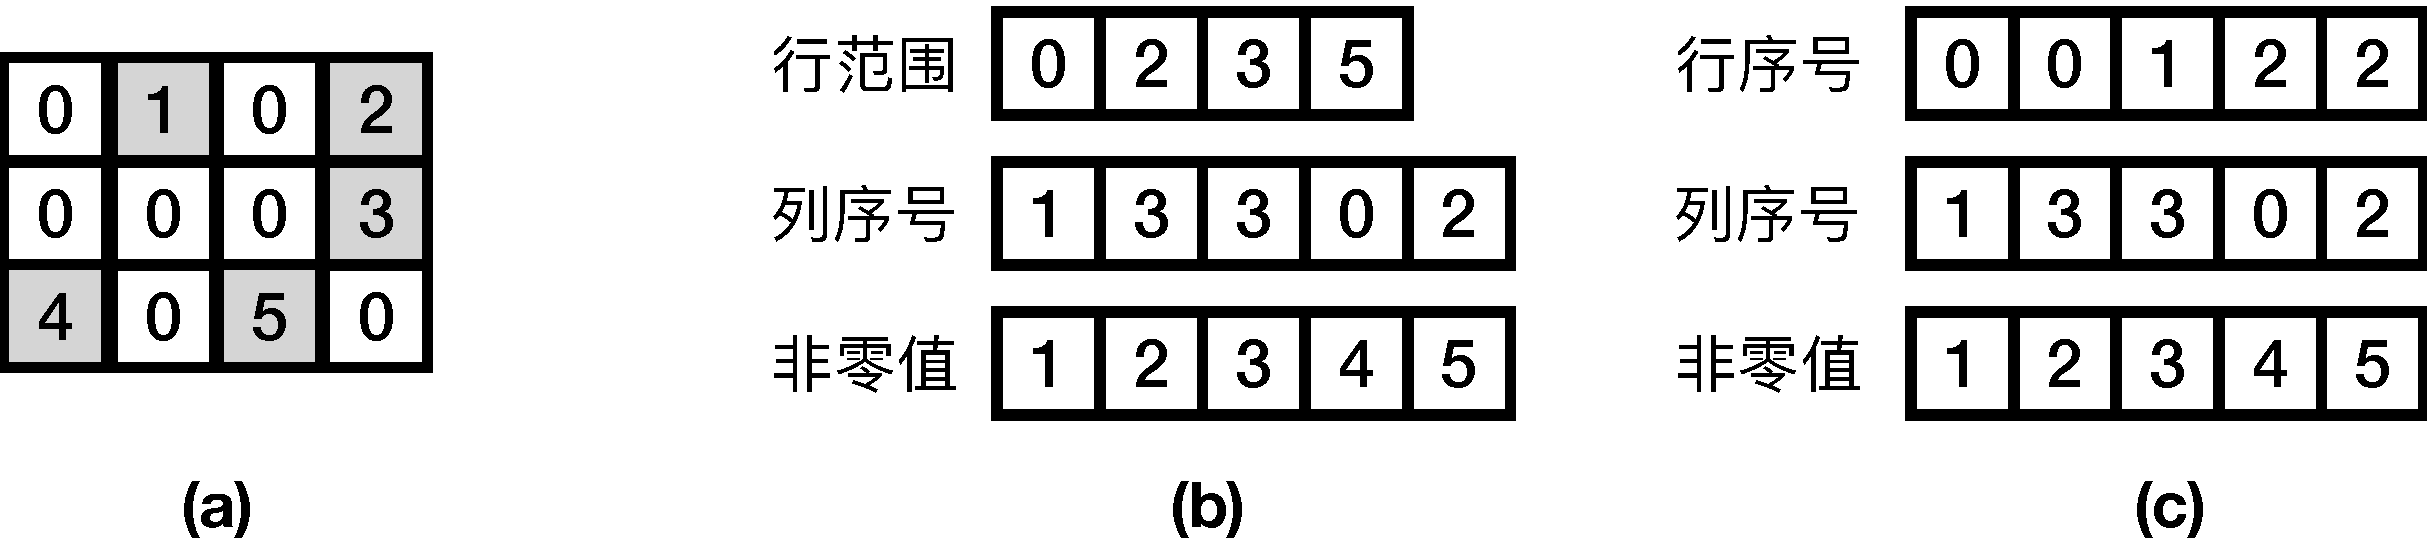
\includegraphics[width=0.99\linewidth]{稀疏矩阵示意图.pdf}
  \caption*{(a)稀疏矩阵;(b)稀疏矩阵压缩稀疏行(CSR)存储格式,由三个数组组成。行范围数组中第$i+1$个元素和第$i$个元素的差值代表第$i$行中非零元个数,列序号数组中第$i$个元素代表第$i$个非零元的列序号,非零值数组中第$i$个元素代表第$i$个非零元的值;
  (c)稀疏矩阵压缩坐标(COO)存储格式,由三个数组组成。行序号数组中第$i$个元素代表第$i$个非零元的行序号,列序号数组中第$i$个元素代表第$i$个非零元的列序号,非零值数组中第$i$个元素代表第$i$个非零元的值。}
  \caption{稀疏矩阵示例}
  \label{fig:sparse-intro}
\end{figure}

\section{稀疏稠密混合代数}
\subsection{定义}
稀疏稠密混合代数是一种稀疏张量代数,它有两种等价的表示形式:一种是张量形式(Tensor formulation,简称TF)如公式\eqref{eq:algebra-view}所示,另一种是数据库形式(Database formulation,简称DF)如公式\eqref{eq:db-view}所示。
在公式\eqref{eq:algebra-view}中,$\symbf{Y}$是输出张量,$\symbf{X^j}$是稠密输入张量,$symbf{A}$是稀疏输入张量。$symbf{A}$是稀疏的意味着至少有一个维度$a_i$是以压缩格式存储的。$y_1, y_2,\cdots,y_M$,$a_1, a_2,\cdots,a_N$,$x_1^j,x_2^j,\cdots,x_{M^j}^j$是属于相同的下标变量集合。$M$是输出张量的维度,$N$是输入稀疏张量的维度,$D$是输入稠密张量的个数,$M^j$是输入稠密张量$\symbf{X^j}$的维度。
在公式\eqref{eq:db-view}中本文使用信息传播描述描述稀疏稠密混合代数。$Q,Q_0,Q_1,Q_2$是向关联数据库的查询。
本文遵循经典的逻辑-物理分离存储思想\cite{codd1970relational}。$D$是$Q$的关联数据库,
按照$id$升序存储$(id, value)$,其中$id\in \mathbb{Z}$,$value \in \mathbb{R}^n$。$dst\in K$是任何可以哈希的键值,$f$是$K\rightarrow \mathbb{Z}$的映射。
$Q(k)$的值定义为$Q(dst)=D(f(dst))$。$\oplus$可以是任何满足交换律的算符,$\otimes$可以是任何可以接受两个对象作为输入,输出一个可被$\oplus$运算的对象。
$\oplus$的结果会被写入$Q$中的$f(dst)$位置。在DF视角下,稀疏稠密混合代数的稀疏性体现在对于所有$dst$,$Q_0(dst)$是分散的。换句话说,$Q_0(i) \bigcap Q_0(i+1) \sim \O$。
该代数的稠密性体现在$D,D_1,D_2$中的值可以是标量,稠密向量或稠密矩阵。
\begin{equation}
  \symbf{Y}_{y_1, y_2,\cdots,y_M} = \symbf{A}_{a_1, a_2,\cdots,a_N}\prod_{i=1}^{D}\symbf{X}^{j}_{x_1^j,x_2^j,\cdot,x_{M^j}^j}
  \label{eq:algebra-view}
\end{equation}
\begin{equation}
  Q(dst)=\oplus_{src\in Q_0(dst)}\{src, \otimes(Q_1(src,dst), Q_2(dst))\}
  \label{eq:db-view}
\end{equation}
在TF下,稀疏稠密混合代数特征是输入既有稀疏又有稠密张量。例如,矩阵化张量乘Khatri-Rao积MTTKRP(Matricized Tensor Times Khatri Rao Product\cite{nisa2019mttkrp},采样稠密矩阵乘法SDDMM(Sampled Dense-Dense Matrix Multiplication)\cite{yu2021exploiting},
稀疏稠密矩阵乘法SpMM(Sparse Matrix-Matrix Multiplication)\cite{huang2020ge}和张量矩阵乘TTM(Tensor Times Matrix Product)\cite{kurt2022ttm}。在TF下,MTTKRP,TTM,SDDMM和SpMM四类算子可以表示为公式\eqref{eq:four-expressions}
\begin{subequations}
  \begin{equation}
      \symbf{Y}_{i,j} = \symbf{A}_{i,k,l}\symbf{X}_{k,j}^1\symbf{X}_{l,j}^2
  \end{equation}
  \begin{equation}
      \symbf{Y}_{i,j,l} = \symbf{A}_{i,j,k}\symbf{X}_{k,l}^1
  \end{equation}
  \begin{equation}
      \symbf{Y}_{i,k} = \symbf{A}_{i,k}\symbf{X}_{i,j}^1\symbf{X}_{j,k}^2
  \end{equation}
  \begin{equation}
      \symbf{Y}_{i,k} = \symbf{A}_{i,j}\symbf{X}_{j,k}^1
  \end{equation}
  \label{eq:four-expressions}
\end{subequations}
\subsection{规约}\label{sec:reduction-core}
稀疏稠密混合代数的核心操作是规约。这一个核心观察启发本文针对规约做优化,因为本文只需要加速这一个核心操作,然后通过编译器技术来自动加速不同的稀疏稠密混合代数。
例如在TF视角下,公式\eqref{eq:algebra-view}算子在MTTKRP的$l,k$维度做规约,TTM在$k$维度,SDDMM在$j$维度,SpMM在$j$维度做规约。规约可以再一个稀疏和一个稠密维度之间进行,比如MTTKRP,TTM和SpMM。
规约也可以在两个稠密维度做,比如SDDMM。图~\ref{fig:kernels}展示了这四种算子的规约维度。本文也在图~\ref{fig:four-code}中给出了规约的具体代码例子。例如,MTTKRP包含两个规约,每个规约都和SpMM中的
规约动作一致。这样的性质也可以在DF视角下观察到。 如图~\ref{fig:redb-spmm}和图~\ref{fig:redb-mttkrp},对于MTTKRP和SpMM的第一个规约,$D_1$的值都是标量,$D_2$的值都是向量。对于MTTKRP的第二个规约,尽管$D_1$的值是一个向量,这一点和SpMM不同,
但是$\oplus$行为一致,因为$\otimes$执行的是向量的逐元素乘法。
\begin{figure}[h]%
  \centering
  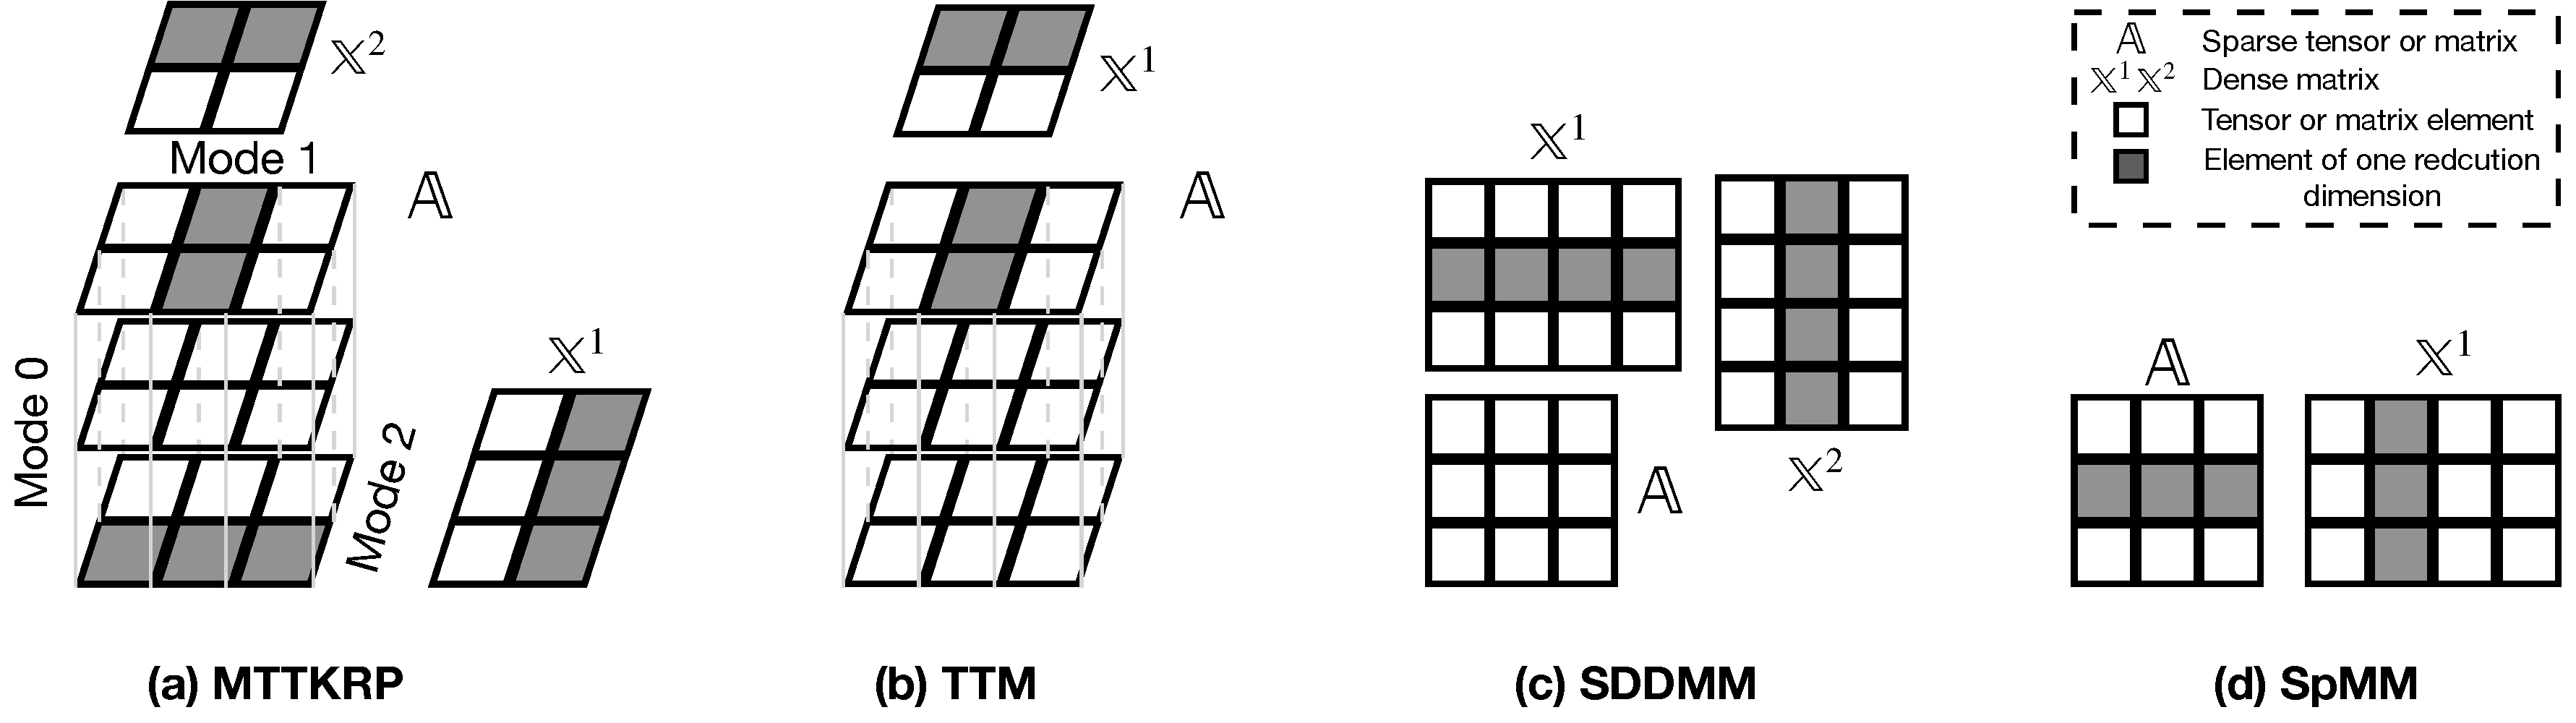
\includegraphics[width=0.99\textwidth]{kernels.pdf}
  \caption{TF视角下稀疏稠密混合代数示例,连续的灰色平行四边形或正方形代表规约维度}
  \label{fig:kernels}
\end{figure}
\begin{figure}[h]%
  \centering
  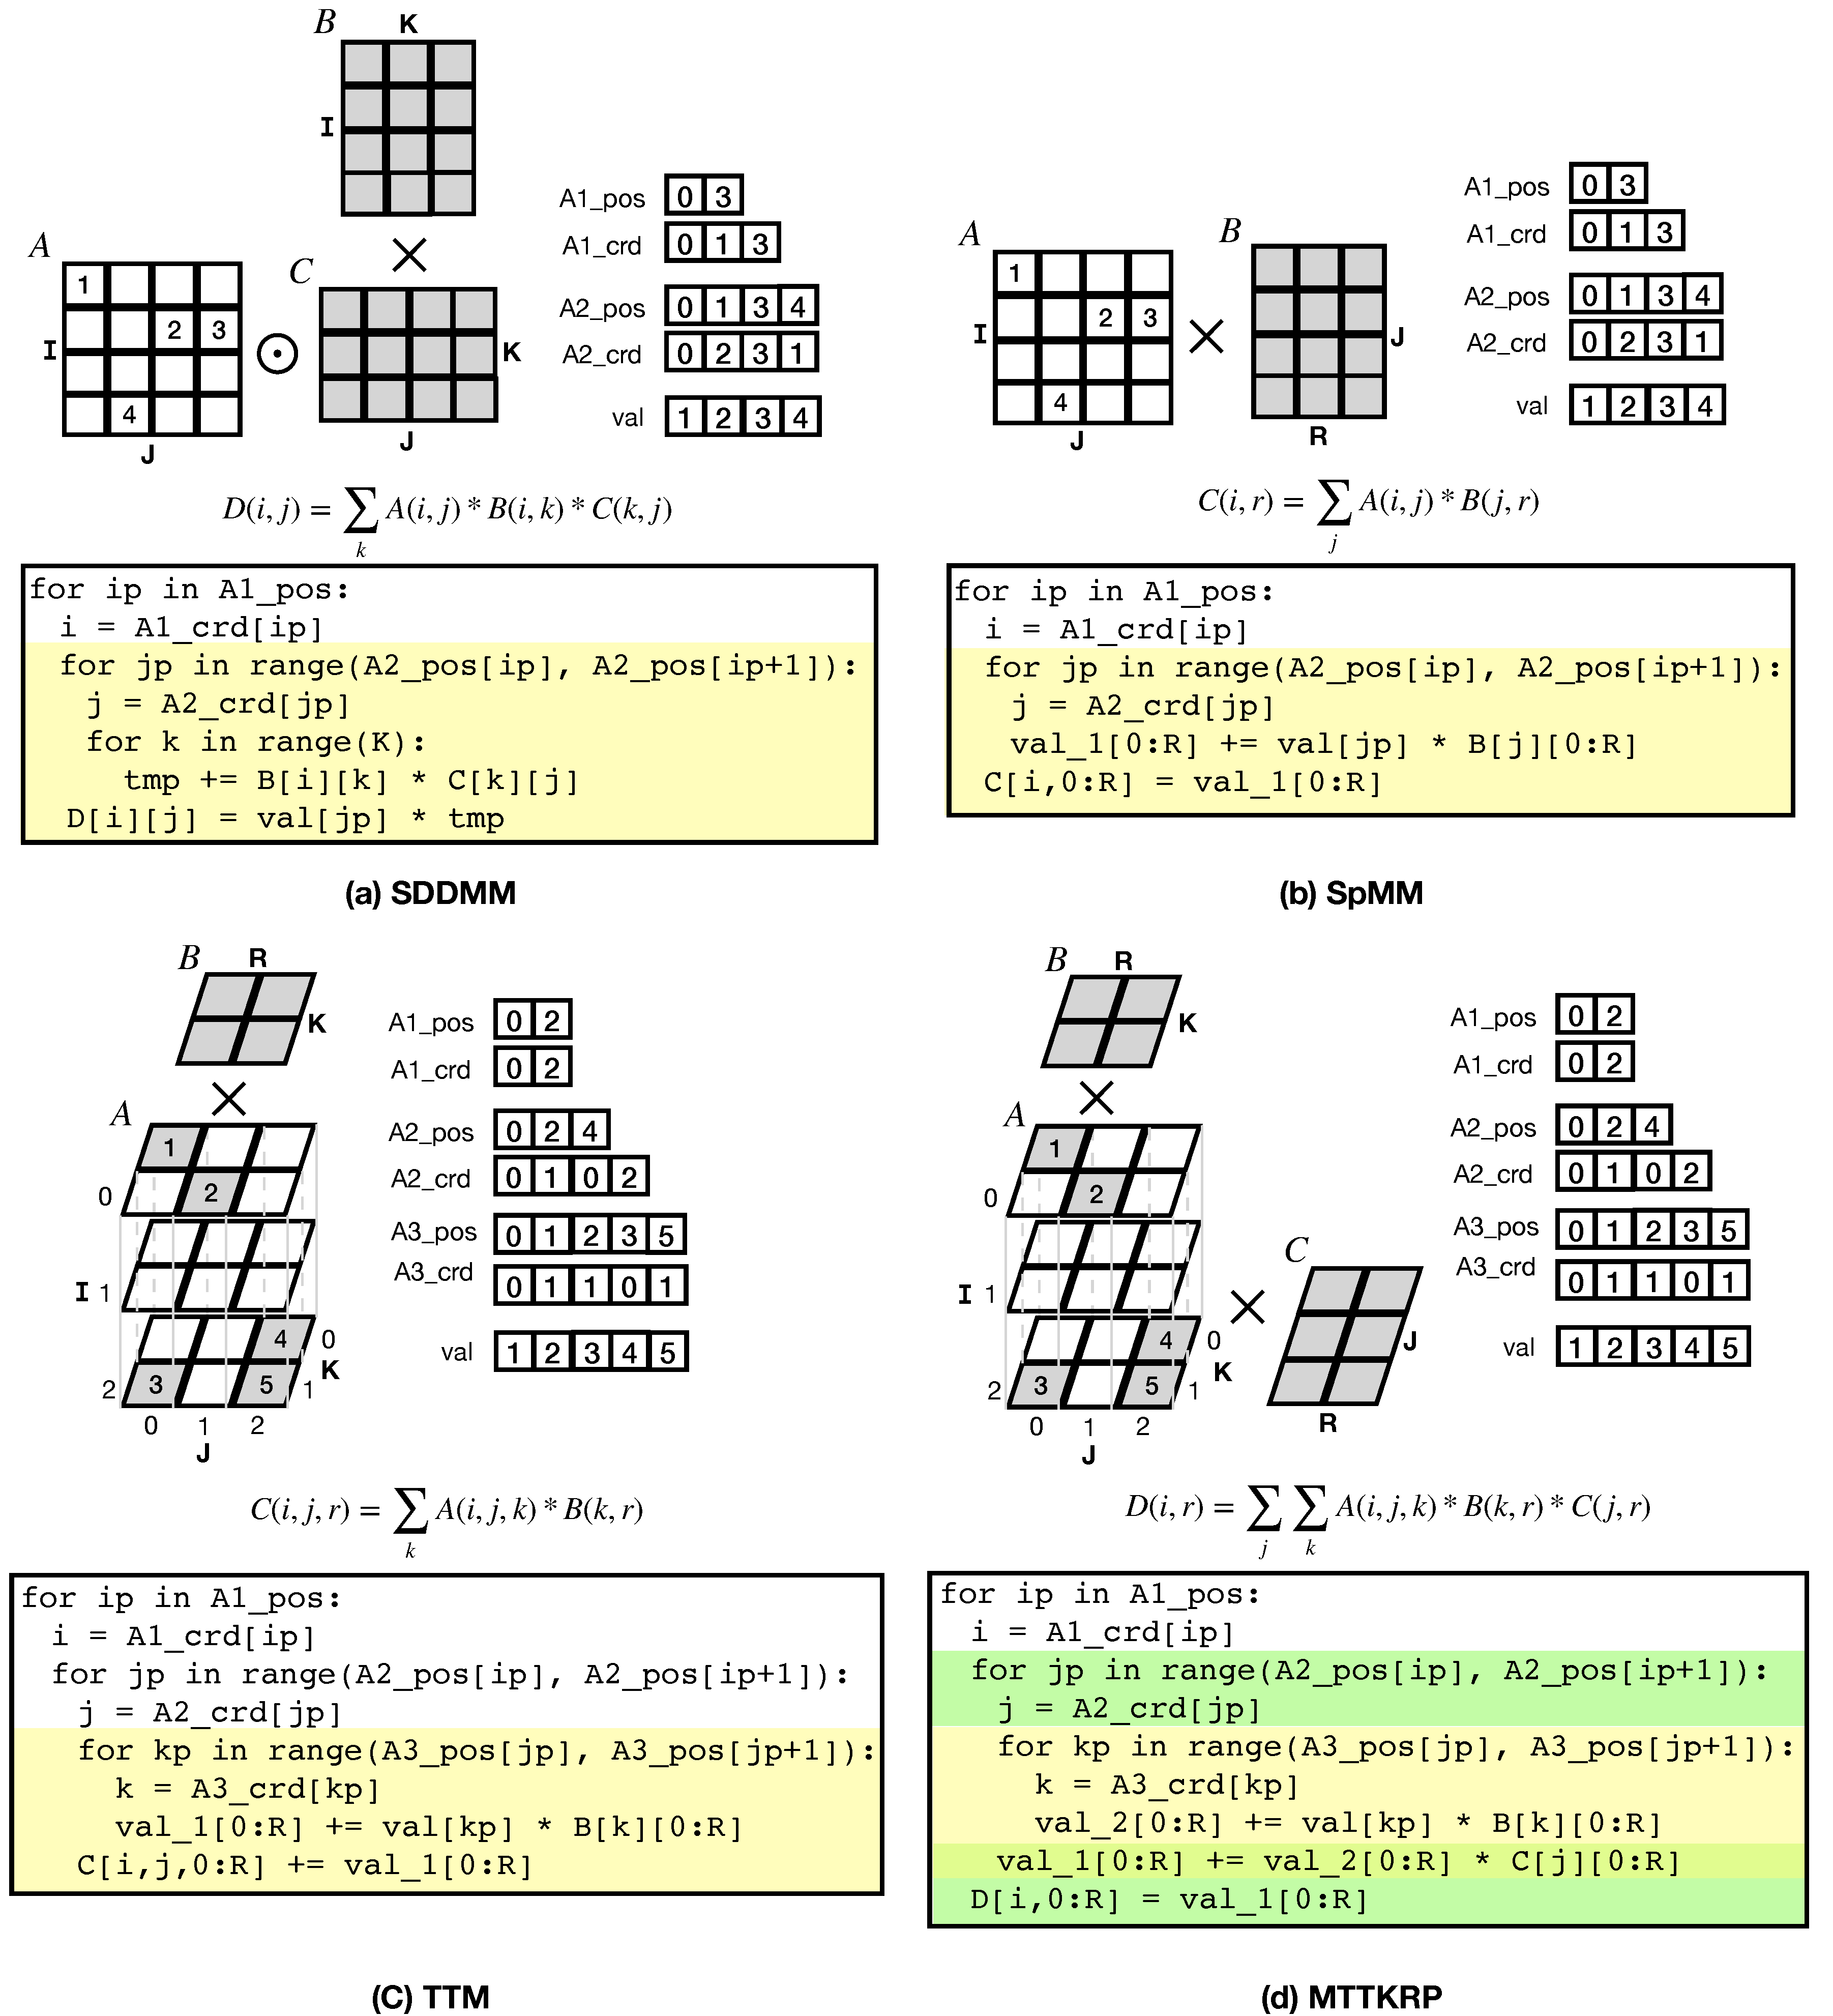
\includegraphics[width=0.99\textwidth]{SpHY.pdf}
  \caption{TF视角下稀疏稠密混合代数规约的代码示例。黄色的和绿色的代码行是规约代码。MTTKRP有两个层次的归于,分别用黄色和绿色表示。重叠部分代表第一个层级的规约输出是第二个层级规约的输入。对于A的存储本文遵循\cite{kjolstad:2020:phd-thesis}的命名规则}
  \label{fig:four-code}
\end{figure}
\begin{figure}[h]%
  \centering
  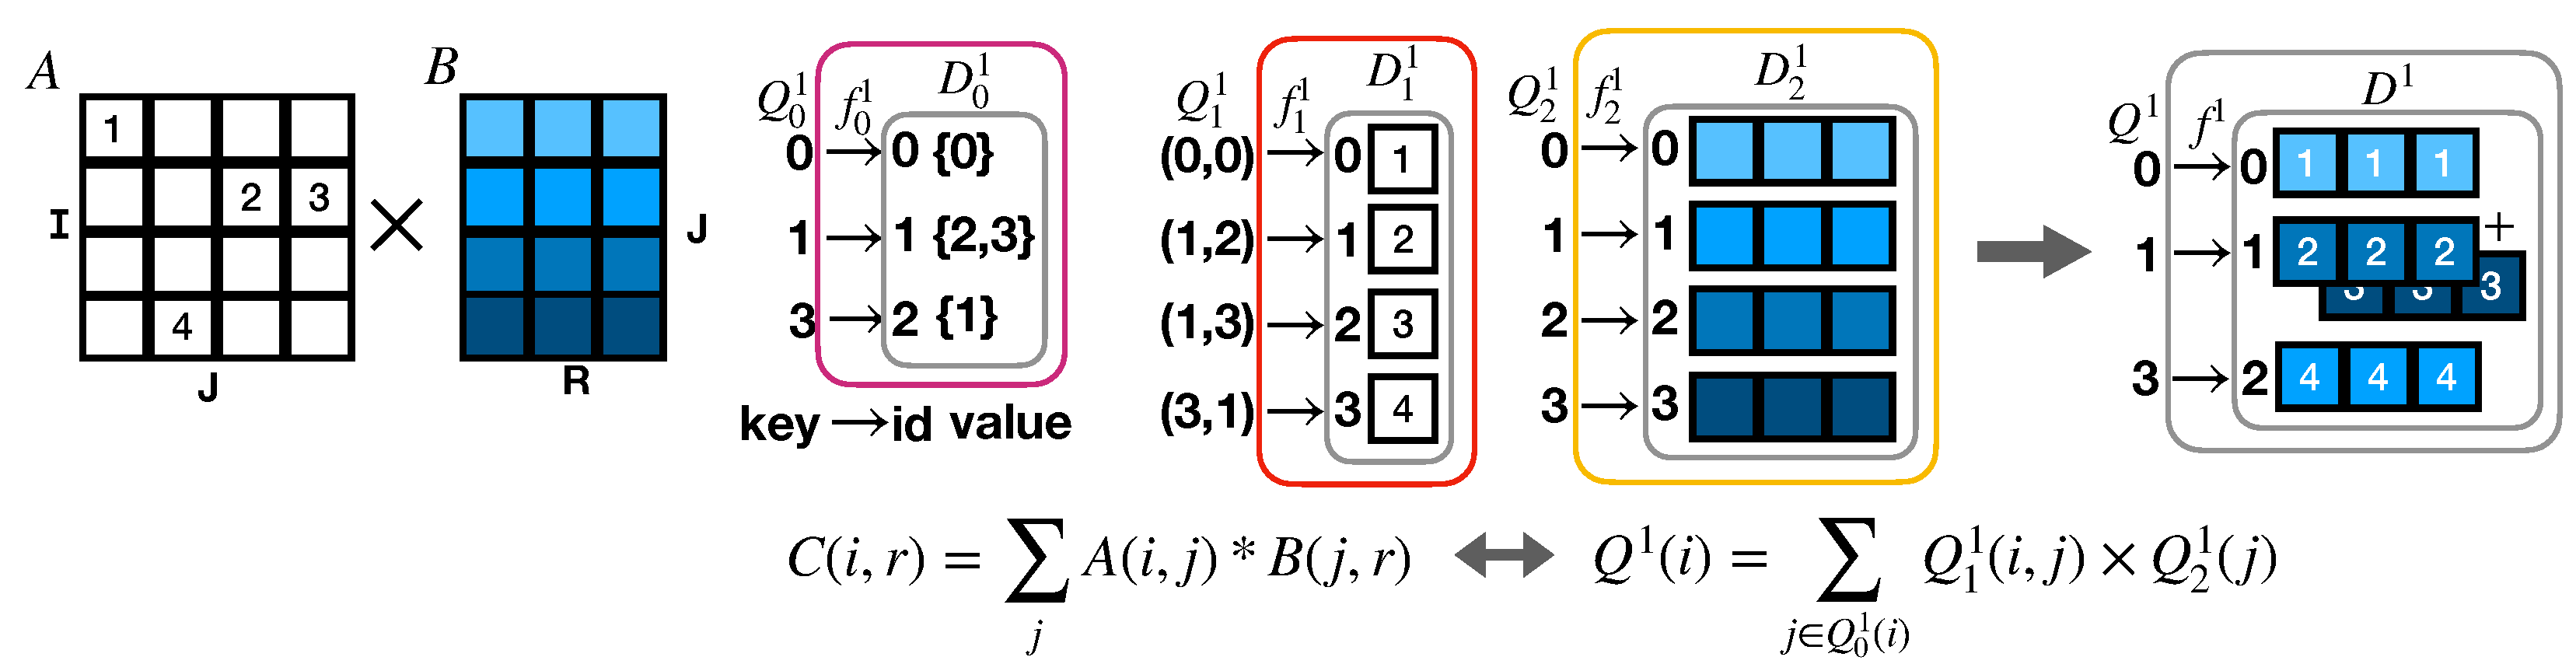
\includegraphics[width=0.99\textwidth]{reduction-db-spmm.pdf}
  \caption{SpMM规约操作示意图,下方展示了该算子在TF和DF视角下等效的表达}
  \label{fig:redb-spmm}
\end{figure}
\begin{figure}[h]%
  \centering
  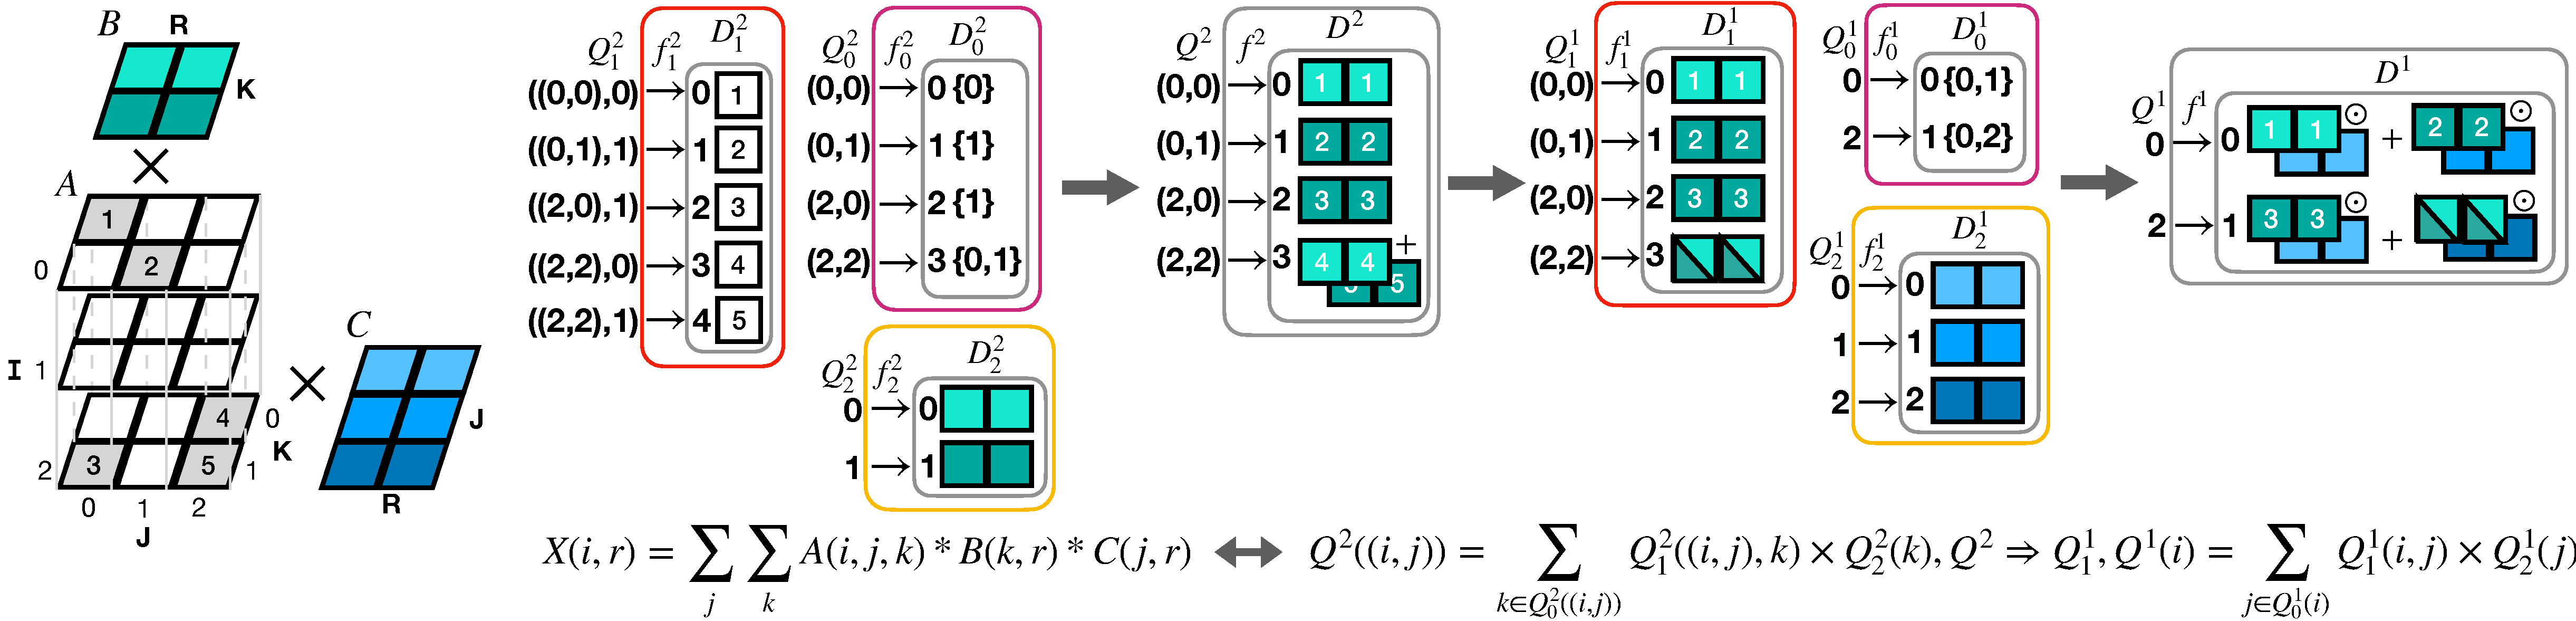
\includegraphics[width=0.99\textwidth]{reduction-db-mttkrp.pdf}
  \caption{MTTKRP规约操作示意图,下方展示了该算子在TF和DF视角下等效的表达}
  \label{fig:redb-mttkrp}
\end{figure}

\section{稀疏稠密张量代数GPU优化技术}\label{sec:spmmopt}
如上节所述,规约是稀疏稠密混合张量代数的核心操作,不同算子之间会共享同类型的规约。因此,不失一般性,本文介绍SpMM在GPU上的算子优化技术。
这些优化技术经过简单扩展就可以应用到其他的稀疏稠密混合代数算子中。Yang等人\cite{yang2018design}通过动态选择两个算法来实现在不同并行处理器中非零元个数的平均分配,和不同线程之间的行平均分配。自适应稀疏切分(ASpT)\cite{hong2019adaptive}通过非零元位置重排实现更好的数据局部性,因此降低了向全局内存的访问次数。
Ge-SpMM\cite{huang2020ge}提出了协调行快取技术(Coalesced Row Caching)来实现向稀疏和稠密矩阵的协调内存访问。同时提出了粗粒度线程组合并技术(Coarse-grained Warp Merging)去合并SpMM在不同线程组的工作负载,并实现更好的稀疏矩阵数据复用。Mehrabi等人\cite{mehrabi2021learning}提出了针对CSR格式的行交换技术来实现更好的工作负载均衡和数据局部性。
DA-SpMM\cite{dai2022heuristic}提出了SpMM的三个设计维度,分别是行/非零元均衡、行/列起始循环,并行/串行规约,并基于机器学习算法设计了自动算子选择器。

\section{稀疏算子编译器}\label{sec:spcomp}
优化稀疏张量代数有四个维度的复杂度:数据格式、代数表达、优化技巧和硬件平台。如前所述,常见数据格式有CSR,CSF,COO,DIA,DCSR,CSB,CSC等,不仅如此,用户还可以根据问题自定义数据格式。
代数表达方面,除了已经列举的SpMM,SDDMM,MTTKRP,TTM等还有更多用爱因斯坦和\cite{einsteinsum}形式表达的张量运算。优化技巧方面,在~\ref{sec:spmmopt}节中本文列举了SpMM的常见优化技巧,
针对其他稀疏算子也会有各自的优化技巧。硬件平台除了CPU,GPU,还会有FPGA和其他的领域专用电路(ASIC)等。通常研究者们会针对一个数据格式、一种张量计算和一个硬件平台开发一系列优化算法。这种研究方式
本文称之为算子模式。算子模式严重依赖于领域专家和大量的工程工作\cite{wang2014mkl,naumov2010cusparse,guennebaud2010eigen}。

但是,稀疏算子编译器有望解决这一问题。它可以降低工程量,并加速这一领域的创新。与算子库模式不同,稀疏算子编译器的目标是用一个整体的编译理论来表述所有数据格式和计算表达,以计算图变换方式表达常用的优化技术,同时希望提出一个灵活的用户接口,这个接口可以让用户针对给定输入数据和硬件平台探索优化空间。稀疏算子编译器的研究可以分为两类。
一类是作为编译器变换步骤。这一类方法会在编译器在高层次语言代码到底层语言代码变换过程中添加稀疏计算相关优化技术的变换。这一类代表工作有Bik和Wijshoff向类FORTRAN语言中添加的编译期数据格式选择技术\cite{bik1993compilation},Venkat等人基于Inspector-Executor模式设计的循环稠密化代码变换技术,以及Strout等人基于多边体模型\cite{polyhedral}提出的稀疏多边体模型\cite{strout2018sparse}。
另一类是作为领域专用语言。这一类方法针对稀疏张量计算设计了专用的高级语言,和从高级语言到底层语言的变换及调度算法\cite{SparseTIR,kjolstad:2020:phd-thesis,bik2022compiler}。特别地,TACO\cite{kjolstad:2017:taco,kjolstad:2019:workspaces,kjolstad:2020:phd-thesis,senanayake:2020:scheduling}针对第二类技术提出了基础算法。据本文所知,它是第一个提出实用稀疏编译理论的工作。MLIR的稀疏方言\cite{bik2022compiler}利用MLIR部署了TACO的稀疏编译理论。SparseTIR\cite{SparseTIR}提出了数据格式融合和混合调度调度策略,但是
它也使用了TACO提出的基础概念,诸如坐标空间和位置空间。同时,TACO还启发了针对稀疏张量代数运算的专用加速器设计\cite{qin2022HardTACO}。因此,本文的工作也基于TACO的编译算法基础。TACO的整体工作流如图~\ref{fig:tacoworkflow}所示。下面,本文将以前端、中端、后端的顺序介绍。
\begin{figure}[h]%
  \centering
  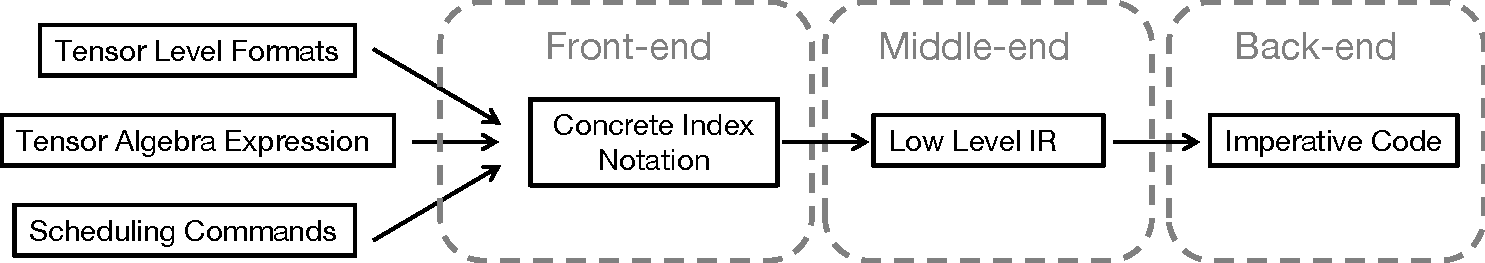
\includegraphics[width=0.9\textwidth]{workflow.pdf}
  \caption{Overview of the TACO workflow}\label{fig:tacoworkflow}
\end{figure}
\subsection{前端}
在前端,稀疏张量表达式被具体化为具象角标表示(Concrete Index Notation,简称CIN)\cite{kjolstad:2019:workspaces}。CIN是一种描述稀疏张量运算执行过程的语言。与爱因斯坦和形式表达的张量运算不同,CIN描述了循环、角标变量之间的关系、转移空间、硬件平台等信息。CIN通过调度指令控制变换。例如一个precompute指令会向CIN中添加where语句。尽管TACO提供了一个简明且有分块、调整循环变量顺序等功能的调度接口来控制CIN变换,但这一调度接口的完备性和有效性还未得到证明\cite{ahrens:2022:autoscheduling}。因此,用户仍然需要直接更改CIN。
TACO中提供了可以接收lambda表达式的匹配函数。这一函数可以更改CIN当它在CIN中寻找到了指定类型的CIN节点或者指定的CIN节点组合模式。不仅如此,TACO还可以通过重载角标表示重写类来直接针对部分CIN进行重写。这个设计帮助本文实现在编译器中部署灵活规约扩展。
\subsection{中端}
在中端,CIN会变换成低层次中间表示(Low Level Intermediate Representation,简称LLIR)。LLIR描述了基本算术操作,变量声明,函数调用等接近C++语言的功能,也包括许多基本块,比如for循环、while循环、if条件语句等。LLIR的下一层就是可执行的C++代码。中端的输出是LLIR序列。基于稀疏迭代理论\cite{kjolstad:2020:phd-thesis}提供的变换规则CIN被变换成LLIR。它保证了不同张量之间只会在可能产生非零输出的元素间循环,这样避免了多余的计算。这也是稀疏张量算子优化的基本原理。特别地,TACO针对CIN中的每一种语句设计了到LLIR的变换函数,同时假设了在稀疏张量的压缩维度上执行的规约是串行,而不是并行。
本文在灵活规约的编译器扩展中会打破串行规约的假设。不仅如此,本文还将指出更灵活的甚至用户可定义的CIN到LLIR变换设计方法可以进一步提升稀疏张量编译器的优化效率。
\subsection{后端}
在后端,LLIR会被直接翻译成不同后端可执行的代码。这篇工作面向英伟达GPU的CUDA代码生成。当前TACO的CUDA代码生成后端有一些文章中没有阐释清楚的限制。TACO用嵌套循环的方式\cite{senanayake:2020:scheduling}将逻辑上串行的LLIR转化为针对单指令多线程(SIMT)的CUDA编程模式。同时,它假设有两层并行单元:线程和线程块,这两层并行单元都是一维的,而CUDA编程模式中并行单元是3维的。这样虽然简化了代码生成算法,却限制了并行编程的写法。当一个for循环LLIR的角标变量被绑定在GPU的线程块时,它会使用blockIdx.x来索引这个角标变量。而在生成CPU代码时,它会生成一个for循环。这样的变量会假设按照1累加。
绑定在GPUWarp和GPUThread上的角标变量分别被假设是threadIdx.x的外部和内部循环变量。TACO默认利用了英伟达GPU中32个线程组成线程组(Warp),并按照线程组粒度调度指令的特性。分块的大小取决于GPUThread上的角标变量。值得注意的是,这里将GPUWarp分块和同步语义混合在了一起,这样导致损失了在GPU线程组维度的灵活调度优化机会。基于这个观察,本文会在本工作中提出分块和同步分离的GPU线程组抽象,并辅助实现灵活规约在稀疏算子编译器的拓展。
